%======================================================================
%  DSA PROJECT DOCUMENTATION
%  Text & Code Plagiarism Detection System in C
%  CS162 – Data Structures and Algorithms
%======================================================================

\documentclass[12pt,a4paper]{article}

% ── Packages ─────────────────────────────────────────────────────────
\usepackage[a4paper, top=2.5cm, bottom=2.5cm, left=2.5cm, right=2.5cm]{geometry}
\usepackage{graphicx}
\usepackage{titlesec}
\usepackage{tocloft}
\usepackage{fancyhdr}
\usepackage{setspace}
\usepackage{enumitem}
\usepackage{xcolor}
\usepackage{booktabs}
\usepackage{array}
\usepackage{tabularx}
\usepackage{longtable}
\usepackage{hyperref}
\usepackage{listings}
\usepackage{float}
\usepackage{tikz}
\usetikzlibrary{shapes.geometric, arrows.meta, positioning}
\usepackage{amsmath}
\usepackage{mdframed}
\usepackage{parskip}
\usepackage{microtype}

% ── Colors ───────────────────────────────────────────────────────────
\definecolor{primaryblue}{RGB}{0,70,127}
\definecolor{accentblue}{RGB}{0,120,215}
\definecolor{lightgray}{RGB}{245,245,245}
\definecolor{codered}{RGB}{180,0,0}
\definecolor{darkgray}{RGB}{60,60,60}
\definecolor{boxblue}{RGB}{230,240,255}
\definecolor{codebg}{RGB}{250,250,250}

% ── Hyperref ─────────────────────────────────────────────────────────
\hypersetup{colorlinks=true, linkcolor=primaryblue,
            urlcolor=accentblue, citecolor=codered}

% ── Section formatting ───────────────────────────────────────────────
\titleformat{\section}[block]
  {\Large\bfseries\color{primaryblue}}{\thesection.}{0.5em}{}
  [\color{accentblue}\titlerule]

\titleformat{\subsection}[block]
  {\large\bfseries\color{darkgray}}{\thesubsection.}{0.5em}{}

\titleformat{\subsubsection}[block]
  {\normalsize\bfseries\color{codered}}{\thesubsubsection.}{0.5em}{}

% ── Header / Footer ──────────────────────────────────────────────────
\pagestyle{fancy}
\fancyhf{}
\rhead{\small\color{darkgray}CS162 – DSA Project Documentation}
\lhead{\small\color{darkgray}Text \& Code Plagiarism Detection System}
\cfoot{\thepage}
\renewcommand{\headrulewidth}{0.4pt}
\renewcommand{\footrulewidth}{0.4pt}

% ── Code listing style ───────────────────────────────────────────────
\lstdefinestyle{cstyle}{
  language=C,
  backgroundcolor=\color{codebg},
  basicstyle=\ttfamily\small,
  keywordstyle=\color{primaryblue}\bfseries,
  commentstyle=\color{darkgray}\itshape,
  stringstyle=\color{codered},
  breaklines=true,
  frame=single,
  framerule=0.6pt,
  rulecolor=\color{accentblue},
  numbers=left,
  numberstyle=\tiny\color{darkgray},
  stepnumber=1,
  tabsize=4,
  showspaces=false,
  showstringspaces=false,
  aboveskip=6pt,
  belowskip=6pt
}
\lstset{style=cstyle}

\lstdefinestyle{bashstyle}{
  language=bash,
  backgroundcolor=\color{lightgray},
  basicstyle=\ttfamily\small,
  keywordstyle=\color{primaryblue},
  frame=single, framerule=0.5pt,
  rulecolor=\color{accentblue},
  numbers=none,
  breaklines=true
}

% ── TikZ for dependency diagram only ─────────────────────────────────
\tikzset{
  mod/.style={rectangle, rounded corners=3pt, draw=primaryblue,
              fill=boxblue, minimum width=2.8cm, minimum height=0.7cm,
              font=\small\ttfamily\bfseries},
  dep/.style={-Stealth, dashed, color=accentblue}
}

%======================================================================
\begin{document}
\onehalfspacing

%──────────────────────────────────────────────────────────────────────
%  PAGE 1 – COVER PAGE
%──────────────────────────────────────────────────────────────────────
\thispagestyle{empty}
\begin{center}

  \vspace*{1cm}
  % ──────────────────────────────────────────────────────────────────
  % INSTITUTE PROFILE PICTURE
  % Replace the fbox below with your institute image:
  %   \includegraphics[width=0.45\textwidth]{institute.png}
  % ──────────────────────────────────────────────────────────────────
  \fbox{%
    \begin{minipage}[c][6cm][c]{9cm}
      \centering
      \textcolor{darkgray}{%
        \large\textbf{[ Institute Profile Picture ]}\\[0.5cm]
        \normalsize Replace this box with:\\[0.3cm]
        \small\texttt{\textbackslash includegraphics[width=0.45\textbackslash textwidth]\{institute.png\}}
      }
    \end{minipage}%
  }

  \vspace{1.0cm}
  {\Huge\bfseries\color{primaryblue}
    Text \& Code\\[0.3cm] Plagiarism Detection System}

  \vspace{0.4cm}
  \color{accentblue}\rule{0.65\textwidth}{1.5pt}\color{black}

  \vspace{0.5cm}
  {\large\bfseries CS162 – Data Structures \& Algorithms\\[0.2cm]
   Project Documentation}

  \vspace{1.0cm}
  \begin{tabular}{ll}
    \textbf{Submitted by:} & \textit{[Your Full Name]}             \\[4pt]
    \textbf{Student ID:}   & \textit{[Your Student ID]}            \\[4pt]
    \textbf{Course:}       & CS162 – Data Structures \& Algorithms \\[4pt]
    \textbf{Instructor:}   & \textit{[Instructor's Name]}          \\[4pt]
    \textbf{Semester:}     & \textit{[e.g.\ Spring 2026]}          \\[4pt]
    \textbf{Date:}         & \textit{\today}
  \end{tabular}

  \vspace{1.2cm}
  \color{accentblue}\rule{0.65\textwidth}{1.5pt}
\end{center}

\newpage

%──────────────────────────────────────────────────────────────────────
%  PAGE 2 – TABLE OF CONTENTS
%──────────────────────────────────────────────────────────────────────
\thispagestyle{fancy}
\renewcommand{\contentsname}{\color{primaryblue}Table of Contents}
\tableofcontents
\newpage

%──────────────────────────────────────────────────────────────────────
%  PAGE 3 – PROJECT TITLE + OBJECTIVE
%──────────────────────────────────────────────────────────────────────

\section{Project Title}

\begin{mdframed}[backgroundcolor=boxblue, linecolor=accentblue,
                 linewidth=1.5pt, innertopmargin=10pt,
                 innerbottommargin=10pt, innerleftmargin=14pt,
                 innerrightmargin=14pt]
  \centering
  {\LARGE\bfseries\color{primaryblue}
    Text \& Code Plagiarism Detection System in C}\\[0.4cm]
  {\normalsize
    A token-based file comparison engine built upon classical\\
    Data Structures: Stack, Hash Table, and Linked List}
\end{mdframed}

\vspace{0.5cm}

This project is the semester capstone for CS162 – Data Structures and Algorithms. It is written entirely in the C programming language and deliberately exercises the core data structure concepts taught throughout the course — stacks, hash tables, and linked lists — to solve the real-world problem of automated plagiarism detection.

\section{Objective / Use of the Project}

\subsection{Purpose}

The primary objective is to build a \textbf{token-based plagiarism detection system} that automatically compares a reference (base) file against one or more other files and reports a numerical similarity score for each pair. Unlike naive character-by-character or exact-string matching, this system captures \emph{semantic similarity} at the word (token) level, making it resilient to common obfuscation tricks such as changing indentation, punctuation, or letter case.

\subsection{Real-World Applications}

Automated plagiarism detection addresses a genuine and growing challenge in academic institutions and the software industry:

\begin{itemize}[leftmargin=1.5cm, itemsep=4pt]
  \item Flag suspicious pairs of student assignments (source code or text essays) without requiring any instructor to read every submission manually.
  \item Allow instructors to focus manual review only on high-similarity pairs flagged by the tool.
  \item Serve as a lightweight, dependency-free alternative to heavyweight commercial tools (e.g., Turnitin, MOSS), suitable for offline or resource-constrained environments.
  \item Work on \emph{any} plain-text file type: C code, Python scripts, Java programs, essays, or any other text document.
  \item Help students self-check their own work before submission to ensure unintentional similarity is not flagged.
\end{itemize}

\subsection{Why Token-Based Comparison?}

Exact-match comparison fails when a student simply reformats code, rearranges lines, or changes letter case. Token-based comparison normalizes each line into a \emph{set of words (tokens)} and measures the Jaccard similarity between those sets. This approach is:

\begin{itemize}[leftmargin=1.5cm, itemsep=4pt]
  \item \textbf{Robust} — insensitive to whitespace, letter case, and punctuation.
  \item \textbf{Efficient} — hash tables provide O(1) average-time token lookup.
  \item \textbf{Mathematically grounded} — the Jaccard index is a well-understood, interpretable similarity metric used in information retrieval and NLP.
  \item \textbf{Extensible} — the modular architecture allows adopting more sophisticated similarity metrics without changing the pipeline.
\end{itemize}

\newpage

%──────────────────────────────────────────────────────────────────────
%  PAGE 4 – INPUT AND OUTPUT
%──────────────────────────────────────────────────────────────────────

\section{Input and Output}

\subsection{Input}

The program is invoked from the command line and accepts the following arguments:

\begin{center}
  \texttt{./detector \textless base\_file\textgreater\
          \textless file1\textgreater\ \textless file2\textgreater\ \ldots}
\end{center}

\begin{table}[H]
\centering
\renewcommand{\arraystretch}{1.5}
\begin{tabularx}{0.94\textwidth}{>{\bfseries\ttfamily}l X}
\toprule
Argument & Description \\
\midrule
base\_file        & The reference (original, authoritative) document.
                    May be a \texttt{.c} source file, \texttt{.py} script,
                    plain text file, or any other text-based format. \\
file1, file2, \ldots & One or more files to compare against the base.
                        The program processes each one in order and prints
                        a separate report for every pair. \\
\bottomrule
\end{tabularx}
\caption{Command-line arguments accepted by the system}
\end{table}

\smallskip
\textbf{Internal compile-time constants} (defined in \texttt{common.h}):

\begin{table}[H]
\centering
\renewcommand{\arraystretch}{1.4}
\begin{tabularx}{0.94\textwidth}{>{\ttfamily\bfseries}l l X}
\toprule
Constant     & Value & Purpose \\
\midrule
TABLE\_SIZE   & 1000  & Number of buckets in each hash table \\
WORD\_LEN    & 50    & Maximum number of characters in one token \\
MAX\_LINE    & 512   & Maximum characters read from a single line \\
THRESHOLD   & 0.5   & Minimum Jaccard score for a line-pair to count as matched \\
\bottomrule
\end{tabularx}
\caption{Global constants from \texttt{common.h}}
\end{table}

\subsection{Expected Output}

For each comparison file the program prints a short three-line report to standard output:

\begin{lstlisting}[style=bashstyle, caption={Sample program output}]
Comparing with file1.c
Matching Lines: 7/10
Similarity: 70.00%
\end{lstlisting}

\begin{itemize}[leftmargin=1.5cm, itemsep=4pt]
  \item \textbf{Comparing with \textit{filename}} — identifies which file was compared.
  \item \textbf{Matching Lines: x/y} — the number of line-pairs whose Jaccard similarity is $\geq 0.5$ out of the total lines read.
  \item \textbf{Similarity: z\%} — overall plagiarism percentage = $(\text{matched} / \text{total}) \times 100$.
\end{itemize}

\newpage

%──────────────────────────────────────────────────────────────────────
%  PAGE 5 – PROCESS FLOW DIAGRAM
%──────────────────────────────────────────────────────────────────────

\section{Process Flow Diagram}

The diagram below illustrates the complete end-to-end pipeline through which input files are transformed into the final similarity report. Each box corresponds to a distinct processing stage, and each stage maps to one or more source-code modules in the project.

\vspace{0.6cm}

% ──────────────────────────────────────────────────────────────────────
% FLOW DIAGRAM IMAGE PLACEHOLDER
% ──────────────────────────────────────────────────────────────────────
% Replace the \fbox block below with:
%   \includegraphics[width=\textwidth]{flowchart.png}
% after adding your flowchart image (flowchart.png) to the project folder.
% ──────────────────────────────────────────────────────────────────────
\begin{figure}[H]
  \centering
  \fbox{%
    \begin{minipage}[c][15cm][c]{0.88\textwidth}
      \centering
      \textcolor{darkgray}{%
        \LARGE\textbf{[ Process Flow Diagram ]}\\[1cm]
        \large Insert your hand-drawn or tool-generated\\
        flow diagram image here.\\[0.8cm]
        \normalsize Replace this placeholder with:\\[0.3cm]
        \texttt{\textbackslash includegraphics[width=\textbackslash textwidth]\{flowchart.png\}}\\[0.8cm]
        \small Suggested tool: draw.io, Lucidchart, or hand-drawn \& scanned.\\[0.4cm]
        The diagram should show the 8 stages:\\[0.3cm]
        Start $\rightarrow$ Open Files $\rightarrow$ Read Line $\rightarrow$
        Normalize $\rightarrow$ Tokenize\\[0.2cm]
        $\rightarrow$ Hash Insert $\rightarrow$ Jaccard $\rightarrow$
        Threshold Check $\rightarrow$ Report $\rightarrow$ End
      }
    \end{minipage}%
  }
  \caption{End-to-end process flow of the Plagiarism Detection System}
\end{figure}

\newpage

%──────────────────────────────────────────────────────────────────────
%  PAGES 6–9 – STEP-BY-STEP EXPLANATION
%──────────────────────────────────────────────────────────────────────

\section{Step-by-Step Explanation}

Each step below includes a full description of what the code does, the underlying algorithmic concept, the data structure(s) used, and the actual source code block from the project.

%---------------------------------------------------------------------
\subsection{Step 1 — Command-Line Argument Parsing (\texttt{main.c})}
%---------------------------------------------------------------------

\textbf{What happens at this stage:}\\
The program begins execution at the \texttt{main()} function in \texttt{main.c}. The operating system passes all command-line arguments through the \texttt{argc} (argument count) integer and the \texttt{argv} (argument vector) array of strings. The function first validates that the user has supplied at least three arguments: the program executable name, the base file, and at least one comparison file. If the validation fails, a descriptive usage message is printed and the program exits cleanly. If the arguments are valid, a \texttt{for} loop iterates from \texttt{argv[2]} through \texttt{argv[argc-1]}, invoking \texttt{compareFiles(argv[1], argv[i])} for each comparison file in sequence.

\smallskip
\textbf{General explanation:}\\
Argument validation is a fundamental defensive programming practice. Without this guard, passing fewer arguments would cause the program to dereference a null or uninitialized pointer, leading to undefined behaviour and a crash. The structured iteration over \texttt{argv} demonstrates how arrays in C can represent a variable-length list of inputs, with simple integer indexing providing O(1) direct access to any element.

\smallskip
\textbf{Data structure used:} \textit{Arrays} — \texttt{argv} is a one-dimensional array of character pointers (C-strings), indexed from 0 to \texttt{argc-1}. Random access into this array is constant-time O(1).

\begin{lstlisting}[caption={\texttt{main.c} -- Entry point, argument parsing, and comparison loop}]
#include "common.h"
#include "compare.h"

int main(int argc, char *argv[]) {

    /* Validate that at least a base file and one compare file
       were provided as command-line arguments.               */
    if (argc < 3) {
        printf("Usage: %s base file1 file2 ...\n", argv[0]);
        return 0;
    }

    /* argv[1] is the base file.
       argv[2] ... argv[argc-1] are the files to compare.   */
    for (int i = 2; i < argc; i++) {
        compareFiles(argv[1], argv[i]);
    }

    return 0;
}
\end{lstlisting}

%---------------------------------------------------------------------
\subsection{Step 2 — File Opening and Line Reading (\texttt{compare.c})}
%---------------------------------------------------------------------

\textbf{What happens at this stage:}\\
The \texttt{compareFiles} function opens both the base file and the comparison file using the standard C \texttt{fopen} call in read mode (\texttt{"r"}). If either file cannot be opened (e.g., the path is wrong or the file does not exist), an error message is printed and the function returns early. The function then enters a \texttt{while} loop that simultaneously reads one line from each file into separate character buffers using \texttt{fgets}. The loop continues as long as both files have remaining lines, processing each matched pair of lines together. Two integer counters, \texttt{matched} and \texttt{total}, are maintained throughout to accumulate the comparison statistics.

\smallskip
\textbf{General explanation:}\\
Reading with \texttt{fgets} is safe and line-oriented: it reads up to \texttt{sizeof(line)-1} characters or until a newline, whichever comes first. The simultaneous dual-file reading pattern (reading both in lock-step) mirrors how a human reviewer scans two documents side by side, comparing structurally corresponding lines. This is appropriate for source code where the overall structure and line ordering carry meaning.

\smallskip
\textbf{Data structure used:} \textit{Character arrays (C-strings)} — \texttt{char line1[MAX\_LINE]} and \texttt{char line2[MAX\_LINE]} are static character arrays of 512 bytes each, allocated on the stack. Two scalar integer counters (\texttt{matched}, \texttt{total}) act as accumulators.

\begin{lstlisting}[caption={\texttt{compare.c} -- File opening and simultaneous line reading}]
void compareFiles(char *file1, char *file2) {

    FILE *f1 = fopen(file1, "r");
    FILE *f2 = fopen(file2, "r");

    /* Guard: exit early if either file could not be opened */
    if (!f1 || !f2) {
        printf("Error opening files\n");
        return;
    }

    char line1[MAX_LINE], line2[MAX_LINE];
    int matched = 0, total = 0;

    /* Read one line from each file simultaneously */
    while (fgets(line1, sizeof(line1), f1) &&
           fgets(line2, sizeof(line2), f2)) {

        /* ... (processing continues in steps 3-7) ... */

        total++;
    }

    fclose(f1);
    fclose(f2);

    /* Step 8: compute and print the final similarity report */
    float percent = (total == 0) ? 0 : (float)matched / total * 100;
    printf("\nComparing with %s\n", file2);
    printf("Matching Lines: %d/%d\n",  matched, total);
    printf("Similarity: %.2f%%\n",     percent);
}
\end{lstlisting}

\newpage

%---------------------------------------------------------------------
\subsection{Step 3 — Text Normalization (\texttt{utils.c})}
%---------------------------------------------------------------------

\textbf{What happens at this stage:}\\
Before any comparison can occur, each raw line must be standardized so that trivially different representations of the same content compare as equal. The \texttt{normalize} function iterates over every character of the input string character by character. It applies two rules: (a) only alphanumeric characters (\texttt{isalnum}) and space characters are kept — all punctuation, brackets, semicolons, newlines, and other symbols are silently discarded; (b) every retained character is converted to its lowercase equivalent via \texttt{tolower}. The resulting clean string is written sequentially into an output buffer, which is null-terminated at the end.

\smallskip
\textbf{General explanation:}\\
Normalization is the most important pre-processing step in any text similarity pipeline. Consider the two strings \texttt{"Hello, World!"} and \texttt{"hello world"}. A raw string comparison reports them as completely different. After normalization both become \texttt{"hello world"} and are identified as identical. In the context of source-code comparison, normalization removes semicolons, braces, operators, and other syntax symbols, leaving only the identifiers and keywords that carry semantic meaning. This prevents a student from trivially defeating the detector by adding extra punctuation.

\smallskip
\textbf{Data structure used:} \textit{Character arrays} — both \texttt{input} and \texttt{output} are C-string arrays. An integer index \texttt{j} functions as a write-pointer advancing only when an accepted character is written. This \textit{in-place array filter} pattern runs in O(n) time where n is the input string length.

\begin{lstlisting}[caption={\texttt{utils.c} -- \texttt{normalize}: discard punctuation, convert to lowercase}]
/*
 * normalize()
 * Strips all non-alphanumeric, non-space characters from 'input'
 * and converts every retained character to lowercase.
 * The result is written into 'output'.
 */
void normalize(char *input, char *output) {
    int j = 0;
    for (int i = 0; input[i]; i++) {
        /* Keep only letters, digits, and spaces */
        if (isalnum(input[i]) || input[i] == ' ')
            output[j++] = tolower(input[i]);
    }
    output[j] = '\0';   /* null-terminate the output */
}
\end{lstlisting}

In \texttt{compare.c}, both lines are normalized before tokenization:

\begin{lstlisting}[caption={\texttt{compare.c} -- Calling normalize on both lines inside the loop}]
    char norm1[MAX_LINE], norm2[MAX_LINE];

    normalize(line1, norm1);   /* normalize base-file line    */
    normalize(line2, norm2);   /* normalize compare-file line */
\end{lstlisting}

%---------------------------------------------------------------------
\subsection{Step 4 — Tokenization Using a Stack (\texttt{utils.c} + \texttt{stack.c})}
%---------------------------------------------------------------------

\textbf{What happens at this stage:}\\
The \texttt{processLine} function accepts a normalized line and extracts individual words (tokens) from it one character at a time, using a \texttt{Stack} as a temporary character buffer. A stack is initialized at the start. The function iterates over every character in the line: if the character is alphanumeric, it is pushed onto the stack. When a delimiter (any non-alphanumeric character, including the null terminator) is met and the stack is non-empty, a complete token has been assembled. The function calls \texttt{stackToWord} to copy the stack contents into a character array, then inserts the resulting word into the hash table via \texttt{insertHash}, and finally clears the stack to start accumulating the next token.

\smallskip
\textbf{General explanation:}\\
The stack serves as an \textit{accumulator} — it collects individual characters one by one until a word boundary is reached, at which point the accumulated characters are harvested as a complete token. This is a natural application of the LIFO structure: characters are pushed in order and read out in the same order (from index 0 to \texttt{top}) by \texttt{stackToWord}, preserving the original left-to-right order of the word. The \texttt{clearStack} call (resetting \texttt{top = -1}) is O(1), making this pipeline extremely efficient.

\smallskip
\textbf{Data structure used:} \textit{Stack} — implemented as a fixed-size character array with an integer \texttt{top} field. Push: O(1). Clear: O(1). Read to word: O(k) where k is token length.

\begin{lstlisting}[caption={\texttt{stack.h} + \texttt{stack.c} -- Stack definition and operations}]
/* ---- stack.h ---- */
typedef struct {
    char data[WORD_LEN];  /* character buffer  */
    int  top;             /* index of top (-1 = empty) */
} Stack;

void initStack(Stack *s);            /* set top = -1       */
void push(Stack *s, char c);         /* add char to top    */
void clearStack(Stack *s);           /* reset top = -1     */
void stackToWord(Stack *s, char *w); /* copy to string     */

/* ---- stack.c ---- */
void initStack(Stack *s)  { s->top = -1; }
void clearStack(Stack *s) { s->top = -1; }

void push(Stack *s, char c) {
    if (s->top < WORD_LEN - 1)
        s->data[++s->top] = c;
}

void stackToWord(Stack *s, char *word) {
    int i;
    for (i = 0; i <= s->top; i++)
        word[i] = s->data[i];
    word[i] = '\0';
}
\end{lstlisting}

\begin{lstlisting}[caption={\texttt{utils.c} -- \texttt{processLine}: tokenize a line using the Stack}]
void processLine(char *line, Node *table[]) {
    Stack s;
    initStack(&s);
    char word[WORD_LEN];

    for (int i = 0; ; i++) {
        if (isalnum(line[i])) {
            push(&s, line[i]);        /* accumulate character  */
        } else {
            if (s.top != -1) {        /* word boundary reached */
                stackToWord(&s, word);
                insertHash(table, word); /* store token in hash */
                clearStack(&s);          /* reset for next word */
            }
            if (line[i] == '\0') break; /* end of line         */
        }
    }
}
\end{lstlisting}

\newpage

%---------------------------------------------------------------------
\subsection{Step 5 — Hash Table Insertion (\texttt{hash.c})}
%---------------------------------------------------------------------

\textbf{What happens at this stage:}\\
Each token produced by \texttt{processLine} is stored in a hash table. The hash table is an array of 1000 \texttt{Node*} pointers, all initialized to \texttt{NULL}. The \texttt{hash} function computes a bucket index for a given word using a \textit{polynomial rolling hash} with base 31: $h = (h \times 31 + c) \bmod 1000$ for each character $c$. Once the index is found, \texttt{insertHash} walks the linked list at that bucket. If the token already exists, its frequency counter is incremented (to support future frequency-aware comparisons). If it does not exist, a new \texttt{Node} is allocated with \texttt{malloc}, the token is copied in with \texttt{strcpy}, the count is set to 1, and the new node is prepended to the front of the linked list — a constant-time insertion strategy.

\smallskip
\textbf{General explanation:}\\
Hashing converts a variable-length string into a small fixed-range integer in O(k) time (where k is the string length), allowing direct array indexing. This is orders of magnitude faster than a sorted list search (O(log n)) or a linear scan (O(n)) when processing hundreds of tokens per file. The polynomial hash with prime base 31 distributes strings uniformly across the 1000 buckets, minimizing collisions. Collisions are resolved by \textit{separate chaining}: each bucket holds the head of a linked list of all words that map to that bucket. The frequency counter (\texttt{count}) field is included for extensibility — future versions could weight the Jaccard score by token frequency.

\smallskip
\textbf{Data structures used:} \textit{Hash Table} (array of Node pointers) + \textit{Linked List} (chaining). Average insertion: O(1). Worst-case: O(n). Lookup: O(1) average.

\begin{lstlisting}[caption={\texttt{hash.h} -- Node structure for the hash table / linked list}]
typedef struct Node {
    char        word[WORD_LEN]; /* stored token          */
    int         count;          /* occurrence frequency  */
    struct Node *next;          /* next node in chain    */
} Node;

unsigned int hash(char *word);
void insertHash(Node *table[], char *word);
int  searchHash(Node *table[], char *word);
void clearTable(Node *table[]);
\end{lstlisting}

\begin{lstlisting}[caption={\texttt{hash.c} -- Hash function and insertion with chaining}]
/* Polynomial rolling hash: h = (h*31 + c) mod TABLE_SIZE */
unsigned int hash(char *word) {
    unsigned int h = 0;
    for (int i = 0; word[i]; i++)
        h = (h * 31 + word[i]) % TABLE_SIZE;
    return h;
}

void insertHash(Node *table[], char *word) {
    unsigned int idx  = hash(word);
    Node        *temp = table[idx];

    /* Walk the chain: if word exists, increment count */
    while (temp) {
        if (strcmp(temp->word, word) == 0) {
            temp->count++;
            return;
        }
        temp = temp->next;
    }

    /* Word not found: allocate a new node and prepend */
    Node *newNode = (Node *)malloc(sizeof(Node));
    strcpy(newNode->word,  word);
    newNode->count = 1;
    newNode->next  = table[idx]; /* prepend to chain    */
    table[idx]     = newNode;
}
\end{lstlisting}

%---------------------------------------------------------------------
\subsection{Step 6 — Jaccard Similarity Calculation (\texttt{utils.c})}
%---------------------------------------------------------------------

\textbf{What happens at this stage:}\\
After both lines have been tokenized and their tokens stored in two separate hash tables (\texttt{t1} for the base line, \texttt{t2} for the comparison line), the \texttt{jaccard} function computes the Jaccard similarity index. The algorithm proceeds in two passes. In the first pass, every token in \texttt{t1} is looked up in \texttt{t2} using \texttt{searchHash}: if found, \texttt{intersection} is incremented; in all cases (found or not), \texttt{unionCount} is incremented because the token is in at least one set. In the second pass, every token in \texttt{t2} that is \emph{not} found in \texttt{t1} is added to \texttt{unionCount} (it belongs to the union but not the intersection). The final score is \texttt{intersection / unionCount}. If both lines were empty, 0 is returned.

\smallskip
\textbf{General explanation:}\\
The Jaccard similarity coefficient $J(A,B) = |A \cap B| / |A \cup B|$ is a standard set-theoretic measure of overlap. A value of 1.0 means both line-token-sets are identical. A value of 0.0 means they share no tokens. The threshold of 0.5 means a line-pair must share more than half of its combined token vocabulary to be counted as ``matching.'' This metric is widely used in information retrieval, NLP, and recommendation systems for document similarity.

\smallskip
\textbf{Data structures used:} \textit{Hash Table} for O(1) average membership queries; \textit{Linked List} traversal within each bucket.

\begin{lstlisting}[caption={\texttt{utils.c} -- \texttt{jaccard}: compute Jaccard similarity between two token sets}]
float jaccard(Node *t1[], Node *t2[]) {
    int intersection = 0, unionCount = 0;

    /* Pass 1: iterate over all tokens in t1 */
    for (int i = 0; i < TABLE_SIZE; i++) {
        Node *temp = t1[i];
        while (temp) {
            /* Check if this token also exists in t2 */
            if (searchHash(t2, temp->word))
                intersection++;
            unionCount++;          /* token is in t1, so in union */
            temp = temp->next;
        }
    }

    /* Pass 2: add tokens in t2 that are NOT in t1 to union */
    for (int i = 0; i < TABLE_SIZE; i++) {
        Node *temp = t2[i];
        while (temp) {
            if (!searchHash(t1, temp->word))
                unionCount++;      /* unique to t2 */
            temp = temp->next;
        }
    }

    if (unionCount == 0) return 0;
    return (float)intersection / unionCount;
}
\end{lstlisting}

In \texttt{compare.c}, the Jaccard score is compared against the threshold:

\begin{lstlisting}[caption={\texttt{compare.c} -- Applying threshold and accumulating match count}]
    float sim = jaccard(t1, t2);

    if (sim >= THRESHOLD)   /* THRESHOLD = 0.5 */
        matched++;

    total++;
\end{lstlisting}

\newpage

%---------------------------------------------------------------------
\subsection{Step 7 — Memory Cleanup (\texttt{hash.c})}
%---------------------------------------------------------------------

\textbf{What happens at this stage:}\\
After the Jaccard score for a line pair has been computed and the match/total counters updated, the two hash tables (\texttt{t1} and \texttt{t2}) must be completely cleared and all dynamically allocated memory freed before the next line pair is processed. The \texttt{clearTable} function iterates over all 1000 buckets. For each bucket, it walks the linked list stored there, freeing each \texttt{Node} with \texttt{free}, and then resets the bucket pointer to \texttt{NULL} so the table is ready for reuse on the next iteration.

\smallskip
\textbf{General explanation:}\\
In C, memory allocated with \texttt{malloc} is never reclaimed automatically — there is no garbage collector. If \texttt{clearTable} were omitted, each iteration of the line-reading loop would allocate new nodes and never release the old ones. Over a file with thousands of lines, this would grow into a catastrophic \textit{memory leak}, eventually exhausting all available heap memory and crashing the program. The two-pointer technique used inside \texttt{clearTable} (storing the current node in \texttt{del} before advancing \texttt{temp}) is the standard safe pattern for traversing and freeing a linked list — accessing \texttt{temp->next} after \texttt{free(temp)} would be \textit{use-after-free}, an undefined behaviour.

\smallskip
\textbf{Data structure used:} \textit{Linked List} — traversed in full to free every node. Time complexity: O(n) where n is the total number of nodes across all buckets.

\begin{lstlisting}[caption={\texttt{hash.c} -- \texttt{clearTable}: free all nodes and reset the hash table}]
void clearTable(Node *table[]) {
    for (int i = 0; i < TABLE_SIZE; i++) {
        Node *temp = table[i];
        while (temp) {
            Node *del = temp;     /* save pointer before advancing */
            temp = temp->next;
            free(del);            /* release heap memory           */
        }
        table[i] = NULL;          /* reset bucket to empty         */
    }
}
\end{lstlisting}

The calls to \texttt{clearTable} inside \texttt{compare.c} after every line comparison:

\begin{lstlisting}[caption={\texttt{compare.c} -- Clearing both hash tables after each line-pair}]
        clearTable(t1);   /* free all nodes in base-line table   */
        clearTable(t2);   /* free all nodes in compare-line table */
\end{lstlisting}

%---------------------------------------------------------------------
\subsection{Step 8 — Final Similarity Report (\texttt{compare.c})}
%---------------------------------------------------------------------

\textbf{What happens at this stage:}\\
Once the \texttt{while}-\texttt{fgets} loop in \texttt{compareFiles} exits (because one or both files have been fully read), the function computes the final overall similarity percentage. It divides the accumulated \texttt{matched} count by \texttt{total} and multiplies by 100 to produce a percentage. The edge case where \texttt{total == 0} (both files were completely empty) is handled by a ternary expression that returns 0\% in that scenario, preventing a division-by-zero fault. The result is printed with two decimal places using the \texttt{\%f} format specifier.

\smallskip
\textbf{General explanation:}\\
Expressing similarity as a human-readable percentage is crucial for usability. A similarity score of 70\% is immediately interpretable by an instructor without requiring knowledge of set theory or the Jaccard formula. The final output provides three complementary views of the result: the name of the comparison file (context), the raw matched-lines ratio (granular detail), and the overall percentage (summary judgment). Together they give the reviewer everything needed to decide whether to investigate a submission further.

\smallskip
\textbf{Data structure used:} Scalar \textit{integer} and \textit{float} variables. No complex data structure is needed at this final reporting stage.

\begin{lstlisting}[caption={\texttt{compare.c} -- Computing and printing the final similarity report}]
    fclose(f1);
    fclose(f2);

    /* Compute percentage; guard against division by zero */
    float percent = (total == 0)
                  ? 0
                  : (float)matched / total * 100;

    printf("\nComparing with %s\n",    file2);
    printf("Matching Lines: %d/%d\n",  matched, total);
    printf("Similarity: %.2f%%\n",     percent);
}
\end{lstlisting}

\newpage

%──────────────────────────────────────────────────────────────────────
%  DATA STRUCTURES USED
%──────────────────────────────────────────────────────────────────────

\section{Data Structures Used}

This section consolidates every data structure applied in the project, with their structural definitions, the stage at which they appear, and their time complexity for each operation.

\subsection{Stack (\texttt{stack.h} / \texttt{stack.c})}

\begin{lstlisting}[caption={Stack type definition -- \texttt{stack.h}}]
typedef struct {
    char data[WORD_LEN];  /* fixed-size character array */
    int  top;             /* -1 when empty              */
} Stack;
\end{lstlisting}

\begin{table}[H]
\centering\renewcommand{\arraystretch}{1.3}
\begin{tabularx}{0.92\textwidth}{>{\bfseries\ttfamily}l X l}
\toprule
Operation & Description & Complexity \\\midrule
initStack    & Set top to -1 (mark as empty)              & O(1) \\
push         & Write character at \texttt{++top}          & O(1) \\
clearStack   & Reset top to -1                            & O(1) \\
stackToWord  & Copy indices 0..top into a C-string        & O(k) \\
\bottomrule
\end{tabularx}
\caption{Stack operations}
\end{table}

\textbf{Used in:} Step 4 (Tokenization — \texttt{processLine}).\\
\textbf{Rationale:} Collects characters one by one into a word; delimiter signals the end of a token.

\subsection{Hash Table with Separate Chaining (\texttt{hash.h} / \texttt{hash.c})}

\begin{lstlisting}[caption={Hash table node -- \texttt{hash.h}}]
typedef struct Node {
    char        word[WORD_LEN]; /* token string      */
    int         count;          /* frequency         */
    struct Node *next;          /* collision chain   */
} Node;

Node *table[TABLE_SIZE];  /* array of 1000 Node pointers */
\end{lstlisting}

\begin{table}[H]
\centering\renewcommand{\arraystretch}{1.3}
\begin{tabularx}{0.92\textwidth}{>{\bfseries\ttfamily}l X l}
\toprule
Operation & Description & Avg.\ Complexity \\\midrule
hash        & Polynomial rolling hash (base 31)         & O(k) \\
insertHash  & Insert or increment token frequency       & O(1) \\
searchHash  & Check if token exists in table            & O(1) \\
clearTable  & Free all nodes; reset all buckets to NULL & O(n) \\
\bottomrule
\end{tabularx}
\caption{Hash table operations}
\end{table}

\textbf{Used in:} Steps 5, 6, 7 (Insert, Jaccard query, Cleanup).\\
\textbf{Rationale:} Near-constant-time insert and lookup across all token comparisons.

\subsection{Linked List (embedded in Hash Table buckets)}

The linked list is not a standalone module but is woven into the hash table through the \texttt{Node*\ next} pointer field. Each hash bucket holds the head of a singly-linked list of all tokens that hash to that bucket.

\textbf{Used in:} Steps 5, 6, 7 — traversal during insertion, search, Jaccard union calculation, and memory cleanup.\\
\textbf{Collision strategy:} Separate chaining.\\
\textbf{Traversal:} O(m) per bucket, where m is the chain length.

\subsection{Arrays}

Arrays appear in multiple roles throughout the project:

\begin{itemize}[leftmargin=1.5cm, itemsep=4pt]
  \item \textbf{Line buffers:} \texttt{char line1[MAX\_LINE]}, \texttt{char line2[MAX\_LINE]}, \texttt{char norm1[MAX\_LINE]}, \texttt{char norm2[MAX\_LINE]} — 512-byte static arrays holding raw and normalized file lines.
  \item \textbf{Token buffers:} \texttt{char word[WORD\_LEN]} — 50-byte arrays holding a single extracted token.
  \item \textbf{Hash table storage:} \texttt{Node *t1[TABLE\_SIZE]}, \texttt{Node *t2[TABLE\_SIZE]} — arrays of 1000 pointers, each the head of a linked-list chain.
  \item \textbf{Argument vector:} \texttt{char *argv[]} — OS-provided array of command-line argument strings.
\end{itemize}

\newpage

%──────────────────────────────────────────────────────────────────────
%  MODULE STRUCTURE
%──────────────────────────────────────────────────────────────────────

\section{Module Structure}

\subsection{File Layout}

\begin{table}[H]
\centering\renewcommand{\arraystretch}{1.5}
\begin{tabularx}{0.96\textwidth}{>{\bfseries\ttfamily}l >{\ttfamily}l X}
\toprule
Header & Source & Responsibility \\\midrule
common.h   & —         & Global macros (\texttt{TABLE\_SIZE}, etc.) and shared \texttt{\#include}s \\
stack.h    & stack.c   & Stack data structure: init, push, clear, stackToWord \\
hash.h     & hash.c    & Hash table + linked list: hash, insert, search, clear \\
utils.h    & utils.c   & normalize, processLine, jaccard \\
compare.h  & compare.c & Orchestrator: compareFiles (calls all other modules) \\
—          & main.c    & Entry point: argument validation, comparison loop \\
\bottomrule
\end{tabularx}
\caption{Module breakdown of the project}
\end{table}

\subsection{Dependency Graph}

\begin{center}
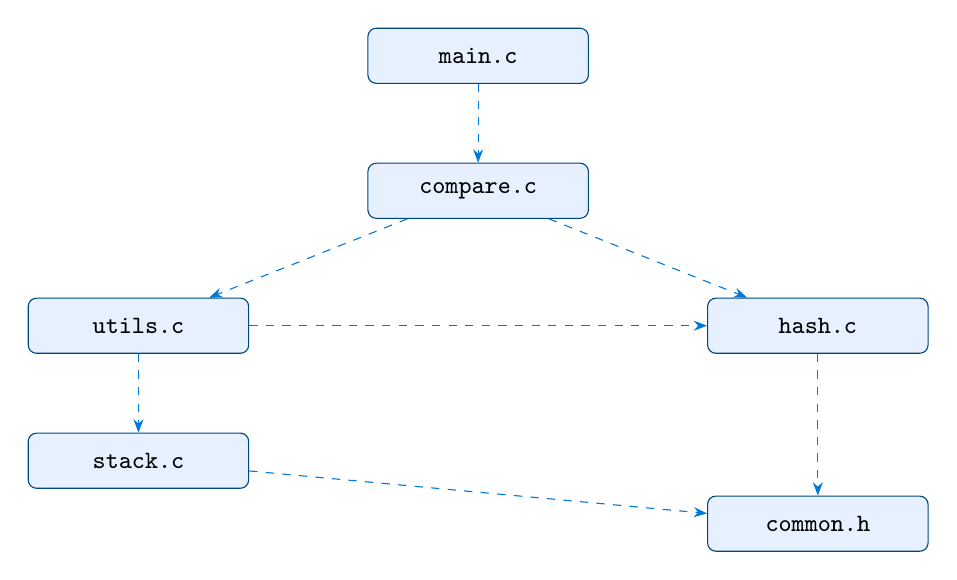
\begin{tikzpicture}[node distance=1.0cm and 1.5cm]
  \node[mod] (main)    {main.c};
  \node[mod, below=of main]   (compare) {compare.c};
  \node[mod, below left=of compare]  (utils)   {utils.c};
  \node[mod, below right=of compare] (hash)    {hash.c};
  \node[mod, below=of utils]          (stack)   {stack.c};
  \node[mod, below=1.8cm of hash]     (common)  {common.h};

  \draw[dep] (main)    -- (compare);
  \draw[dep] (compare) -- (utils);
  \draw[dep] (compare) -- (hash);
  \draw[dep] (utils)   -- (stack);
  \draw[dep] (utils)   -- (hash);
  \draw[dep] (stack)   -- (common);
  \draw[dep] (hash)    -- (common);
\end{tikzpicture}
\end{center}

\subsection{Compilation Command}

\begin{lstlisting}[style=bashstyle, caption={Compile the project with GCC}]
gcc main.c compare.c hash.c stack.c utils.c -o detector
\end{lstlisting}

\textbf{Note:} Do \emph{not} include \texttt{base.c}, \texttt{file1.c}, or \texttt{file2.c} — those are stand-alone test programs, each with their own \texttt{main()}.

\subsection{Sample Run}

\begin{lstlisting}[style=bashstyle, caption={Running on Windows PowerShell}]
.\detector.exe base.c file1.c file2.c
\end{lstlisting}

\begin{lstlisting}[style=bashstyle, caption={Example output}]
Comparing with file1.c
Matching Lines: 5/8
Similarity: 62.50%

Comparing with file2.c
Matching Lines: 3/8
Similarity: 37.50%
\end{lstlisting}

\newpage

%──────────────────────────────────────────────────────────────────────
%  LEARNING OUTCOMES
%──────────────────────────────────────────────────────────────────────

\section{Learning Outcomes}

\subsection{What I Learned from the Project}

Building this plagiarism detection system from scratch in C was a comprehensive exercise that went far beyond writing code. The project forced the integration of theoretical knowledge from lectures into a real, working application.

\begin{enumerate}[leftmargin=1.8cm, label=\textbf{\arabic*.}, itemsep=8pt]

  \item \textbf{Applying Data Structures to Real Problems}\\
  Before this project, stacks and hash tables were abstract concepts studied in isolation. Implementing them within a working application made their trade-offs tangible. I experienced first-hand why O(1) hash lookup matters when processing thousands of tokens across hundreds of lines, and how a simple stack elegantly solves the character-accumulation sub-problem in tokenization.

  \item \textbf{Modular Software Design in C}\\
  Refactoring a monolithic prototype into six distinct modules taught me the value of separation of concerns. Each module can be compiled, tested, and reasoned about independently. I learned to use header guards (\texttt{\#ifndef HEADER\_H}) and include-only-what-you-need discipline to keep dependency graphs clean and understandable.

  \item \textbf{Manual Memory Management}\\
  C has no garbage collector. Writing and debugging \texttt{clearTable} — including the two-pointer safe-free pattern — taught me careful heap discipline. Every \texttt{malloc} must be paired with a \texttt{free}. Forgetting even one leads to a memory leak that only manifests under load, which is a classic systems-programming pitfall. This experience deepened my appreciation for safe memory management in modern languages.

  \item \textbf{Text Pre-Processing and Normalization}\\
  Writing the \texttt{normalize} function revealed how noisy raw text input is. Even a simple filtering step — remove punctuation, lowercase everything — dramatically improves match quality. This gave me a practical foundation in text pre-processing, the first stage in any natural language processing (NLP) pipeline.

  \item \textbf{Similarity Metrics and Thresholds}\\
  Implementing the Jaccard index from its mathematical formula and tuning the threshold (0.5) to balance precision and recall was a rewarding exercise in bridging theory and engineering. Changing the threshold has a direct, observable impact on detection sensitivity — a concept central to machine learning and information retrieval.

  \item \textbf{Command-Line Interfaces and File I/O}\\
  Using \texttt{argc}/\texttt{argv} for flexible multi-file input and \texttt{fgets} for safe, bounded line reading are foundational C skills that apply to virtually every systems or tooling program. These are the building blocks of compilers, shells, database utilities, and countless other tools.

\end{enumerate}

\subsection{What I Learned from the CS162 Course}

The CS162 course provided the theoretical and conceptual foundation that made this project possible, and demonstrated that data structures are not just academic constructs but practical engineering tools.

\begin{enumerate}[leftmargin=1.8cm, label=\textbf{\arabic*.}, itemsep=8pt]

  \item \textbf{Fundamental Data Structures}\\
  The course introduced and analyzed arrays, linked lists, stacks, queues, trees, heaps, hash tables, and graphs. Understanding the internal mechanics — not just the API — of each structure allowed me to implement them correctly from scratch and choose the right one for each sub-problem in this project.

  \item \textbf{Algorithm Complexity Analysis}\\
  The O-notation framework gave me a systematic way to compare algorithms. When choosing between a linear scan and hash lookup for token search, I could justify the decision with a concrete complexity argument: O(n) vs.\ O(1). This analytical thinking is transferable to any programming problem.

  \item \textbf{Hash Tables and Collision Resolution}\\
  The course material on polynomial hashing, load factors, and separate chaining directly informed the implementation of \texttt{hash.c}. Understanding why a prime base (31) distributes strings evenly and why chaining is robust for variable-length-key maps was directly applicable knowledge.

  \item \textbf{Pointer Arithmetic and Dynamic Memory}\\
  CS162 provided a rigorous treatment of pointers, pointer arithmetic, \texttt{malloc}/\texttt{free}, and pointer-based structure traversal — all of which are indispensable in C. Without this foundation, implementing the hash table with linked-list chaining would have been extremely error-prone.

  \item \textbf{Problem Decomposition and Pipeline Design}\\
  Perhaps the most transferable skill from CS162 is the habit of decomposing a complex problem into a pipeline of well-defined, independently testable algorithmic steps. This project's eight-step pipeline (read $\to$ normalize $\to$ tokenize $\to$ hash $\to$ compare $\to$ threshold $\to$ clear $\to$ report) is a direct application of this design methodology.

\end{enumerate}

\vspace{1.2cm}
\begin{center}
  \color{accentblue}\rule{0.65\textwidth}{1pt}\\[0.4cm]
  {\large\bfseries\color{primaryblue} End of Project Documentation}\\[0.2cm]
  \color{accentblue}\rule{0.65\textwidth}{1pt}
\end{center}

\end{document}
